\chapter{YOLO}
\label{sec:yolo}
\ac{yolo} ist ein populäres Objekt Erkennungsmodell, dass dafür bekannt ist besonders schnell und akkurat Objekte in Bildern zu erkennen. Dies liegt an der kleinen Modellgröße und den hohen Berechnungsgeschwindigkeiten. Des Weiteren nutzt \ac{yolo} das gesamte Bild als Trainingsgrundlage, was es sowohl ermöglicht Videos zu klassifizieren als auch die Fehlerrate reduziert, dass der Hintergrund als Teil des Objektes klassifiziert wird. In diesem Kapitel geht es darum wie die Schnittstelle bzw. der Algorithmus gefüttert werden muss und was der Algorithmus für Datenformate erwartet \cite{Jiang.2022}.

\begin{wrapfigure}{r}{5cm}
    \includegraphics[width=4cm]{data/img/ordnerstruktur_yolo.png}
    \caption{Ordnerstruktur für einen Datensatz}
    \label{fig:folderYolo}
\end{wrapfigure}

Für die Studienarbeit wird der YOLOv5 von ultralytics \cite{glennjocher.2023} genommenm, da diese folgende Vorteile bietet:
\begin{itemize}
    \item aktive Developer am Projekt
    \item große Community 
    \item Docker deployable
    \item CUDA- und GPU-Unterstützung
    \item Pytorch Beschleungigung
    \item viele Tutorials und Ressourcen für das Erlernen des Algorithmus
\end{itemize}


\section{Generelle Ordnerstruktur}
\label{sec:yolo_folderstructure}
Der \ac{yolo}-Algorithmus erwartet eine gewisse Ordnerstruktur. Diese muss eingehalten werden, damit der Algorithmus funktioniert. Ein Diagramm der Ordnerstruktur ist zu sehen in \autoref{fig:folderYolo}. Der hierarchisch gesehen höchste Ordner ist der Projektordner. Darin sollten alle Daten für den YOLO-Algorithmus enthalten sein. Dieser Ordner enthält die Trainings- und Testdateien. Optional kann auch ein Validierungsdatensatz enthalten sein und die \textit{.yaml} Datei.

Es wird empfohlen die \textit{.yaml} Datei in den Projektordner zu inkludieren. Der Aufbau der Datei wird in \autoref{sec:yaml_class} genauer beschrieben. Alle Dateien sind innerhalb des Projektordners einzugliedern.

Der Test, Train und Validordner müssen alle jeweils 2 Ordner besitzen mit dem Namen \textit{images} und \textit{labels}. Diese müssen auch über die verschiedenen Ordner exakt gleich, inklusive der Groß- und Kleinschreibung benannt sein.

Der \textit{images} Ordner enthält die entsprechenden Bilder. Zum Trainieren akzeptiert der \ac{yolo}-Algorithmus unter anderem die Bildformate \textit{png},\textit{jpg} und \textit{tiff}. Innerhalb des Ordners müssen alle Bilder einen einzigartigen Namen besitzen (es wird an dieser Stelle empfohlen, alle Bilder durchzunummerieren)

Der \textit{labels}-Ordner enthält die Label zu den entsprechenden Bildern in \textit{images}. Dabei müssen alle Label für ein entsprechendes Bild in einer gleichnamigen Textdatei mit der Endung \textit{.txt} unter dem Ordner \textit{labels} abgespeichert werden. Ein Beispiel: In dem Trainingsordner im Unterordner \textit{images} gibt es ein Bild mit dem Namen \textit{test.jpg}. Die dazugehörige Labeldatei wird im Ordner \textit{labels} unter dem Namen \textit{test.txt} gespeichert.

Im folgenden Abschnitt sollen nun der Aufbau einer solchen Labeldatei erläutert werden.

\section{Aufbau der Labeldatei}
Eine Labeldatei ist wie in \autoref{sec:yolo_folderstructure} definiert eine Textdatei mit entsprechendem Dateiname. Es wird empfohlen die Datei UTF-8 zu enkodieren. 

Jede Datei besteht aus einer unterschiedlichen Anzahl an Zeilen. Jede Zeile der Datei beschreibt ein Objekt, das in der Abbildung zu sehen ist. Es ist möglich, dass diese Bildbereiche eiinander überlappen. Eine Zeile ist wie folgt aufgebaut:
\begin{tcolorbox}
    \begin{verbatim}
        <class> <x-center> <y-center> <width> <height>
    \end{verbatim}
\end{tcolorbox}
\begin{figure}
    \begin{center}
        \includegraphics[width=8cm]{data/img/yolo_picture_structure.png}    
        \caption{Struktur YOLO Format veranschaulicht}
        \label{fig:yoloFormat}
    \end{center}
\end{figure}
\begin{itemize}
    \item \textless class\textgreater gibt die Klasse an des markierten Objektes. Klassen werden durch die \textit{.yaml}-Datei definiert. Gekennzeichnet wird diese durch eine Zahl. Weiteres in \autoref{sec:yaml_class}
    \item \textless x-center\textgreater $\rightarrow$ Angabe des Zentrums des Rechteckes in x-Richtung 
    \item \textless y-center\textgreater $\rightarrow$ Angabe des Zentrums des Rechteckes in y-Richtung 
    \item \textless width\textgreater $\rightarrow$ die Breite des Rechteckes bzw. des markierten Bereiches
    \item \textless height\textgreater $\rightarrow$ die Höhe des Rechteckes bzw. des markierten Bereiches
\end{itemize}
Ein Beispiel ist zu sehen in \autoref{fig:yoloFormat}. \textit{x\_center, y\_center, width, height} werden dargestellt als Verhältnis zur Gesamtlänge/-breite. Die Zahlen sind definiert durch $n\in[0,1]$.

Die Klassen werden im \textit{.yaml} Dateiformat definiert. Diese wird im folgenden Abschnitt genauer beleuchtet.

\section{YAML Klassifizierungsfile}
\label{sec:yaml_class}

Für jedes Projekt gibt es im Projektordner eine \textit{.yaml} Datei mit einem beliebigen Namen. Die \textit{.yaml}-Datei muss allerdings einem gewissen Aufbau folgen der folgend gezeigt wird. Dabei muss die Ordnerstruktur eingehalten werden wie in \autoref{fig:folderYolo} gezeigt:
\begin{verbatim}
    path: <path-to-project>
    train: <rel-path-to-train-dir>
    val: <rel-path-to-val-dir>

    names:
        0: <name>
        ...
\end{verbatim}
\begin{itemize}
\item \textless path-to-project\textgreater  $\rightarrow$ Absoluter Pfad zum Projektordner (inklusive des Projektordners)
\item \textless rel-path-to-train-dir\textgreater  $\rightarrow$ relativer Pfad zu den Bildern des Trainingsdatensatz ausgehend vom \textless path-to-project\textgreater-Pfad
\item \textless rel-path-to-val-dir\textgreater  $\rightarrow$ relativer Pfad zu den Bildern des Validierungsdatensatz ausgehend vom \textless path-to-project\textgreater-Pfad
\item \textit{names} $\rightarrow$ Liste aller Klassen und der Verbindung zwischen Name der Klasse angegeben durch \textless name\textgreater  und der Nummer. Die Nummer, beginnend mit 0 muss auch äquivalent sein zu der Nummerierung in den Textdateien. Der \ac{yolo}-Algorithmus assoziiert die Namen mit den Nummern durch die \textit{.yaml}-Datei
\end{itemize}
